%%%%%%%%%%%%%%%%%%%%%%%% ExtendedAbstract.tex %%%%%%%%%%%%%%%%%%%%%%%%
%                                                                    %
%  Template for the 10-page extended abstract to be submitted for    %
%  the MSc degree conferral at Instituto Superior Tecnico.           %
%                                                                    %
%  Author:                                                           %
%                                                                    %
%       Andre C. Marta                                               %
%       Area Cientifica de Mecanica Aplicada e Aeroespacial          %
%       Departamento de Engenharia Mecanica                          %
%       Instituto Superior Tecnico                                   %
%       Av. Rovisco Pais                                             %
%       1049-001 Lisboa                                              %
%       Portugal                                                     %
%       Tel: +351 21 841 9466                                        %
%                        3466 (extension)                            %
%       Email: andre.marta@ist.utl.pt                                %
%                                                                    %
%  Created:       Dec  2, 2011                                       %
%  Last Modified: Dec 27, 2011                                       %
%%%%%%%%%%%%%%%%%%%%%%%%%%%%%%%%%%%%%%%%%%%%%%%%%%%%%%%%%%%%%%%%%%%%%%
% This document uses the LaTeX class file "article.cls"              %
%%%%%%%%%%%%%%%%%%%%%%%%%%%%%%%%%%%%%%%%%%%%%%%%%%%%%%%%%%%%%%%%%%%%%%
\documentclass[10pt,a4paper]{article}

%%%%%%%%%%%%%%%%%%%%%%%%%%%%%%%%%%%%%%%%%%%%%%%%%%%%%%%%%%%%%%%%%%%%%%
% Document preamble
%%%%%%%%%%%%%%%%%%%%%%%%%%%%%%%%%%%%%%%%%%%%%%%%%%%%%%%%%%%%%%%%%%%%%%


\usepackage{amsmath}
\usepackage{amssymb}
\usepackage{amsfonts}
\usepackage{mathtools}

\usepackage[thmmarks, amsmath]{ntheorem}

\usepackage{graphicx}
\usepackage{xcolor}
\usepackage{float}

\usepackage{tikz}
\usetikzlibrary{arrows, positioning, intersections}
\usepackage{tikz-cd}

\usepackage{diffcoeff}
\diffdef{}{op-symbol=\mathrm{d},op-order-sep=0mu,}
\diffdef{p}{left-delim=\left.,right-delim=\right|,subscr-nudge=0mu}

\usepackage{cancel}
\usepackage{interval}
\usepackage{mleftright}

\usepackage[inline]{enumitem}
\SetEnumitemKey{algorithm}{label={Step \Roman*.}, ref=\Roman*, labelindent=0pt, labelsep=!, leftmargin=*, align=left,itemindent=0pt}
\setlist[enumerate,1]{label=\roman*)}

%\usepackage{showlabels}


\usepackage[pdftex]{hyperref} % enhance documents that are to be
                              % output as HTML and PDF
\hypersetup{colorlinks,       % color text of links and anchors,
                              % eliminates borders around links
%            linkcolor=red,    % color for normal internal links
            linkcolor=black,  % color for normal internal links
            anchorcolor=black,% color for anchor text
%            citecolor=green,  % color for bibliographical citations
            citecolor=black,  % color for bibliographical citations
%            filecolor=magenta,% color for URLs which open local files
            filecolor=black,  % color for URLs which open local files
%            menucolor=red,    % color for Acrobat menu items
            menucolor=black,  % color for Acrobat menu items
%            urlcolor=cyan,    % color for linked URLs
            urlcolor=black,   % color for linked URLs
	          bookmarks=true,         % create PDF bookmarks
	          bookmarksopen=false,    % don't expand bookmarks
	          bookmarksnumbered=true, % number bookmarks
	          pdftitle={Thesis},
            pdfauthor={Duarte Maia},
            pdfsubject={Thesis Title},
            pdfkeywords={Thesis Keywords},
            pdfstartview=FitV,
            pdfdisplaydoctitle=true}

% 'hypcap' package
%
% Adjusting the anchors of captions.
% http://www.ctan.org/tex-archive/macros/latex/contrib/oberdiek/
%
% > fixes the problem with hyperref, that links to floats points
%   below the caption and not at the beginning of the float.
%
\usepackage[figure,table]{hypcap}
\usepackage{sectsty}
\newcommand{\myFontSize}{\fontsize{10}{0}\selectfont}
\sectionfont{\myFontSize}       % 10pt, Bold face (default)
\subsectionfont{\rm\myFontSize} % 10pt, Plain face

%margins
\setlength{\topmargin}{-10.4mm}
\setlength{\headheight}{0.0mm}
\setlength{\headsep}{10.0mm}
\setlength{\textwidth}{160mm}
\setlength{\textheight}{242mm}
\setlength{\oddsidemargin}{0mm}
\setlength{\evensidemargin}{0mm}
\setlength{\marginparwidth}{0mm}
\setlength{\marginparsep}{0mm}
% ----------------------------------------------------------------------
% Define new commands to assure consistent treatment throughout document
% ----------------------------------------------------------------------



\theorembodyfont{\upshape}
\theoremseparator{.}
\newtheorem{theorem}{Theorem}
\renewtheorem*{theorem*}{Theorem}
\newtheorem{prop}{Proposition}
\renewtheorem*{prop*}{Proposition}
\newtheorem{corollary}{Corollary}
\newtheorem{lemma}{Lemma}
\newtheorem{definition}{Definition}
\newtheorem{remark}{Remark}

\theoremstyle{break}
\theorembodyfont{\upshape}
\theoremseparator{.}
\theoremindent0.5cm
\newtheorem{algorithm}{Algorithm}

\theoremstyle{nonumberplain}
\theoremheaderfont{\itshape}
\theorembodyfont{\upshape}
\theoremseparator{:}
\theoremsymbol{\ensuremath{\blacksquare}}
\theoremindent0cm
\newtheorem{proof}{Proof}

\theoremsymbol{\ensuremath{\text{\textit{(End proof of lemma)}}}}
%\theoremsymbol{\ensuremath{\square}}
\newtheorem{lemmaproof}{Proof of lemma}

%Sets of numbers
\newcommand{\R}{\mathbb{R}}
\newcommand{\C}{\mathbb{C}}
\newcommand{\Z}{\mathbb{Z}}

\newcommand{\FF}{\mathbb{F}} %Arbitrary field

%Contractible orbits
\newcommand{\LL}{\mathrm{L}}
%Action functional
\renewcommand{\AA}{\mathrm{A}}
%Generic Barcode
\newcommand{\BB}{\mathrm{B}}

%Floer Complex and Homology
\newcommand{\CF}{\mathrm{CF}}
\newcommand{\HF}{\mathrm{HF}}

\newcommand{\moduli}{M}


\DeclareMathOperator{\Ham}{Ham}

%Morse Complex
\newcommand{\MC}{\mathrm{C}}

\newcommand{\HH}{\mathrm{H}}

\DeclareMathOperator{\Ind}{Ind}
\DeclareMathOperator{\hessian}{Hess}
\DeclareMathOperator{\jacobian}{J}
\newcommand{\Lie}{L}

\newcommand{\I}{\mathrm{i}}
\newcommand{\e}{\mathrm{e}}


\DeclareMathOperator{\sign}{sign}
\let\Im\relax
\DeclareMathOperator{\Im}{Im}
\let\Re\relax
\DeclareMathOperator{\Re}{Re}

\newcommand{\Ix}{\mathop{\mathrm{I\mkern0.7mu x}}}
%\newcommand{\Ix}{\mathop{\mathrm{ix}}}


\newcommand{\id}{\mathrm{id}}

\DeclareMathOperator{\image}{im}


\DeclareMathOperator{\inte}{int}
\DeclareMathOperator{\codim}{codim}
\newcommand{\grad}{\nabla}
\newcommand{\into}{\mathbin{\lrcorner}}

\DeclarePairedDelimiter{\norm}{\lvert}{\rvert}
\DeclarePairedDelimiter{\Norm}{\lVert}{\rVert}
\DeclarePairedDelimiter{\abs}{\lvert}{\rvert}
\DeclarePairedDelimiter{\braket}{\langle}{\rangle}

\newcommand{\conj}[1]{\overline{#1}}
\newcommand{\transposed}{\top}
\DeclareMathOperator{\trace}{Tr}

%conley zehnder index a la hofer and kriener
\newcommand{\muhk}{\mu_{\mathrm{HK}}}
\newcommand{\murs}{\mu_{\mathrm{RS}}}


%%%%%%%%%%%%%%%%%%%%%%%%%%%%%%%%%%%%%%%%%%%%%%%%%%%%%%%%%%%%%%%%%%%%%%%%%%%%%%%%%%%%%%%%
% Title, authors and addresses

\title{Computing Maslov Indices in Two Dimensions and Filtered Floer Homology of a few Hamiltonians on the Torus}
\date{July 2022}
\author{Duarte Maia \\ duarte.nascimento@tecnico.ulisboa.pt\\
\smallskip
Supervisor: Miguel Abreu\\
\\ Instituto Superior T\'{e}cnico, Lisboa, Portugal}

%%%%%%%%%%%%%%%%%%%%%%%%%%%%%%%%%%%%%%%%%%%%%%%%%%%%%%%%%%%%%%%%%%%%%%%%%%%%%%%%%%%%%%%%
\begin{document}


\maketitle

%%%%%%%%%%%%%%%%%%%%%%%%%%%%%%%%%%%%%%%%%%%%%%%%%%%%%%%%%%%%%%%%%%%%%%
% ABSTRACT & KEYWORDS
%%%%%%%%%%%%%%%%%%%%%%%%%%%%%%%%%%%%%%%%%%%%%%%%%%%%%%%%%%%%%%%%%%%%%%
%%%%%%%%%%%%%%%%%%%%%%%%%%%%%%%%%%%%%%%%%%%%%%%%%%%%%%%%%%%%%%%%%%%%%%
%     File: ExtendedAbstract_abstr.tex                               %
%     Tex Master: ExtendedAbstract.tex                               %
%                                                                    %
%     Author: Andre Calado Marta                                     %
%     Last modified : 2 Dez 2011                                     %
%%%%%%%%%%%%%%%%%%%%%%%%%%%%%%%%%%%%%%%%%%%%%%%%%%%%%%%%%%%%%%%%%%%%%%
% The abstract of should have less than 500 words.
% The keywords should be typed here (three to five keywords).
%%%%%%%%%%%%%%%%%%%%%%%%%%%%%%%%%%%%%%%%%%%%%%%%%%%%%%%%%%%%%%%%%%%%%%

%%
%% Abstract
%%
\begin{abstract}


The filtered Floer homology of a symplectic manifold $M$ (satisfying certain technical restrictions) is essentially a version of Floer homology which is parametrized by the actions of the orbits. This makes it a finer invariant than usual Floer homology, at the cost of dependence on the Hamiltonian chosen to calculate it. However, some independence can be recovered, and so filtered Floer homology can be said to be an invariant of Hamiltonian diffeomorphisms. There is already a body of literature on the subject, which is an active area of research, but there are very few concrete examples of filtered Floer homology being computed for particular Hamiltonian diffeomorphisms. In this thesis, we compute the filtered Floer homology of a couple of classes of Hamiltonian diffeomorphisms on the torus. In the process, we give a practical method for computation of Maslov/Conley-Zehnder indices.

\noindent{{\bf Keywords:}} symplectic geometry, persistence homology, floer homology, maslov index, conley-zehnder index
 \\


\end{abstract}



%%%%%%%%%%%%%%%%%%%%%%%%%%%%%%%%%%%%%%%%%%%%%%%%%%%%%%%%%%%%%%%%%%%%%%
% INTRODUCTION
%%%%%%%%%%%%%%%%%%%%%%%%%%%%%%%%%%%%%%%%%%%%%%%%%%%%%%%%%%%%%%%%%%%%%%
%%%%%%%%%%%%%%%%%%%%%%%%%%%%%%%%%%%%%%%%%%%%%%%%%%%%%%%%%%%%%%%%%%%%%%%
%     File: ExtendedAbstract_intro.tex                               %
%     Tex Master: ExtendedAbstract.tex                               %
%                                                                    %
%     Author: Andre Calado Marta                                     %
%     Last modified : 27 Dez 2011                                    %
%%%%%%%%%%%%%%%%%%%%%%%%%%%%%%%%%%%%%%%%%%%%%%%%%%%%%%%%%%%%%%%%%%%%%%
% State the objectives of the work and provide an adequate background,
% avoiding a detailed literature survey or a summary of the results.
%%%%%%%%%%%%%%%%%%%%%%%%%%%%%%%%%%%%%%%%%%%%%%%%%%%%%%%%%%%%%%%%%%%%%%

\section{Introduction}
\label{sec:intro}

\paragraph{Persistence Homology}

\paragra


%%%%%%%%%%%%%%%%%%%%%%%%%%%%%%%%%%%%%%%%%%%%%%%%%%%%%%%%%%%%%%%%%%%%%%
% MAIN
%%%%%%%%%%%%%%%%%%%%%%%%%%%%%%%%%%%%%%%%%%%%%%%%%%%%%%%%%%%%%%%%%%%%%%
% !TeX root = ExtendedAbstract.tex

\section{Persistence Homology}

\nocite{polterovich}

Persistence homology is a tool developed around 1992 for the purpose of data science. Data scientists had the need to compute the homology of a shape given a finite collection of data points $X$, which raises the question of finding a shape which adequately describes the data. A primitive algorithm consists of picking a positive number $r$ and replacing each data point by a sphere of radius $r$. The resulting open set, denoted $X^{(r)}$, may be understood as an approximation of the real shape underlying the data $X$, and there are efficient algorithms to compute its homology.

\begin{figure}
\centering
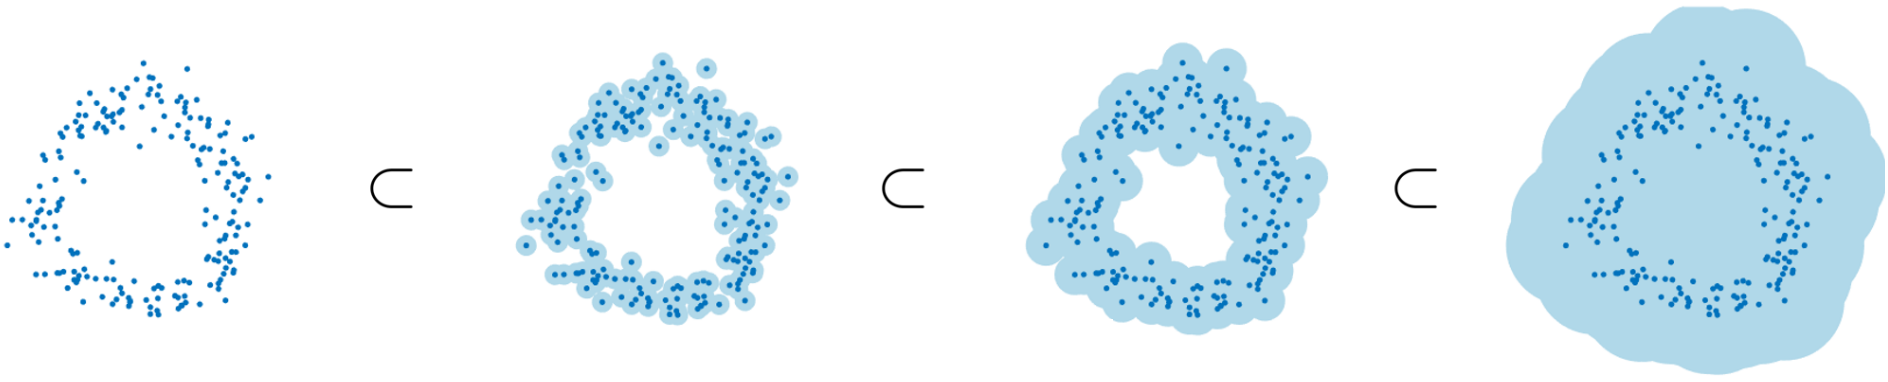
\includegraphics[width=\linewidth]{data}
\caption{Illustration of the sets $X^{(r)}$, with increasing $r$. Note that the middle radii are the ones which better represent the topology of the data. Figure taken from \cite{historypersistence}.}
\end{figure}

This raises the question of which radius $r$ to pick, which requires careful analysis of the data: too small $r$ and the datapoints will be disconnected, too large $r$ and the dataset degenerates into a large ball. However, persistence homology offers an alternative: consider all positive radii at once.

For $k \in \Z$ and $r > 0$, define $H_k^r(X) = H_k(X^{(r)})$, and for $r \leq 0$ set $H_k^r(X) = 0$. These spaces allow us to visualize how the shape of $X^{(r)}$ changes as $r$ increases. Moreover, for $r < s$ the inclusion $X^{(r)} \subseteq X^{(s)}$ induces a natural map $H_k^r(X) \to X_k^s(X)$. This data forms an object which is called a \emph{persistence module}. In the sequence we will be working exclusively with vector spaces, so assume that the homology is taken with coefficients over a field $\FF$.

\begin{definition}
A persistence module is a family of vector spaces $\{V_t\}_{t \in \R}$ (over a field $\FF$), together with maps $\pi_{st} \colon V_s \to V_t$ for $s \leq t$, such that
\begin{align}
\pi_{tt} &= \id,\\
\pi_{tr} \circ \pi_{st} &= \pi_{sr}, \quad s \leq t \leq r.
\end{align}

Moreover, a persistence module $(\{V_t\}_{t \in \R}, \{\pi_{st}\}_{s\leq t})$ is said to be of \emph{finite type} if the following three conditions are satisfied:
\begin{enumerate}
\item For all but finitely many $t$ there exists a neighborhood $U$ of $t$ such that $\pi_{st}$ is an isomorphism for $s, t \in U$,
\item For all $t \in \R$ there exists $\varepsilon$ such that $\pi_{(t-\delta), t}$ is an isomorphism for all $0 \leq \delta < \varepsilon$,
\item\label{pm3} For all $t \in \R$ close enough to $-\infty$, $V_t = 0$.
\end{enumerate}
\end{definition}

In practice, all the constructions for persistence modules that will be discussed in this thesis originate persistence modules of finite type. This is useful because of an important representation theorem for this class of persistence modules. We now introduce the relevant concepts.

\begin{definition}
A \emph{barcode} is a finite multiset\footnote{A multiset is a set whose elements are counted with multiplicity.} of intervals of type $\linterval a b$, with $-\infty < a < b \leq +\infty$. We work under the convention that $\linterval a \infty = \ointerval a \infty$.
\end{definition}

\begin{definition}
Let $B = \{I_1, \dots, I_n\}$ be a barcode. Define the persistence module $\FF(B) = (\{V_t\}_{t \in \R}, \{\pi_{st}\}_{s \leq t})$ as follows
\begin{itemize}
\item Define $V_t = \braket{i \mid t \in I_i}$, where the brackets denote the free vector space over $\FF$,
\item For $s \leq t$, define $\pi_{st} \colon V_s \to V_t$ by defining it on the basis elements of $V_s$. For every $i$ such that $s \in I_i$,
\begin{itemize}
\item If $t \in I_i$, set $\pi_{st}(i) = i$,
\item Otherwise, set $\pi_{st}(i) = 0$.
\end{itemize}
\end{itemize}

It is straight-forward to prove that $\FF(B)$ is a persistence module of finite type.
\end{definition}

\begin{theorem}[Normal Form Theorem]
Every persistence module of finite type is isomorphic to $\FF(B)$ for exactly one barcode $B$.
\end{theorem}

The normal form theorem is the persistence analogous to the classical theorem in linear algebra that says that every vector space of finite dimension is isomorphic to $\R^n$ for some unique $n$. By property \ref{pm3} of finite type persistence modules, every persistence module `starts out' as the zero vector space, and at some instant in time it `grows a new basis element'. This marks the start of a bar in its barcode. Similarly, whenever the vector space $V_t$ loses a dimension, that is marked by the end of a bar. In this sense, the barcode of a persistence module is an indicator of when dimensions are appearing and disappearing; when applied to the homology of a topological space, \emph{the bars mark the appearance and disappearance of holes in the space as the parameter varies}.


\section{Floer Homology}
\label{sec:ph}

Floer homology was developed by Andreas Floer in 1988 in order to attack the so-called Arnol'd conjecture, an important problem in symplectic geometry.


%%%%%%%%%%%%%%%%%%%%%%%%%%%%%%%%%%%%%%%%%%%%%%%%%%%%%%%%%%%%%%%%%%%%%%
% REFERENCES
%%%%%%%%%%%%%%%%%%%%%%%%%%%%%%%%%%%%%%%%%%%%%%%%%%%%%%%%%%%%%%%%%%%%%%

% Produces the bibliography section when processed by BibTeX
%
% Bibliography style
% > entries ordered alphabetically
%\bibliographystyle{plain}
% > unsorted with entries appearing in the order in which the citations appear.
%\bibliographystyle{unsrt}
% > entries ordered alphabetically, with first names and names of journals and months abbreviated
\bibliographystyle{abbrv}
% > entries ordered alphabetically, with reference markers based on authors' initials and publication year
%\bibliographystyle{alpha}

% External bibliography database file in the BibTeX format (ExtendedAbstract_ref_db.bib)
\bibliography{bibliography}

%%%%%%%%%%%%%%%%%%%%%%%%%%%%%%%%%%%%%%%%%%%%%%%%%%%%%%%%%%%%%%%%%%%%%%
\end{document}
%%%%%%%%%%%%%%%%%%%%%%%%%%%%%%%%%%%%%%%%%%%%%%%%%%%%%%%%%%%%%%%%%%%%%%

